\section{The simulation of muons in the SiD detector}
\label{Detector}

In the first step of simulating the muons in the SiD detector, event displays were made with WIRED4.

\begin{figure}
    \centering
    \begin{subfigure}[b]{0.49\textwidth}
    \centering
        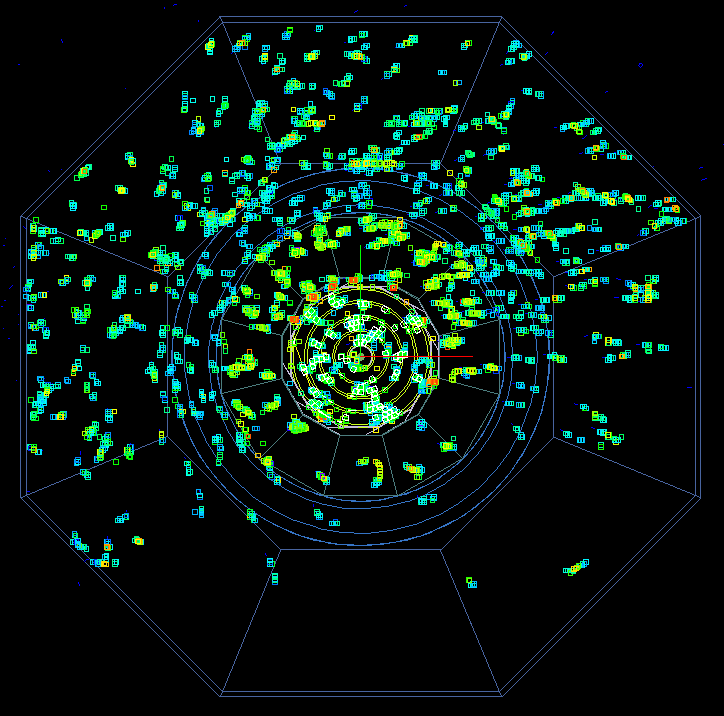
\includegraphics[height=0.3\textheight]{figures/muons_positron_5spoilers_wall_515_xyview_croped.png}
        \caption{xy-view}
	\label{fig:xy_5Spoilers}
    \end{subfigure}
    \begin{subfigure}[b]{0.49\textwidth}
    \centering
        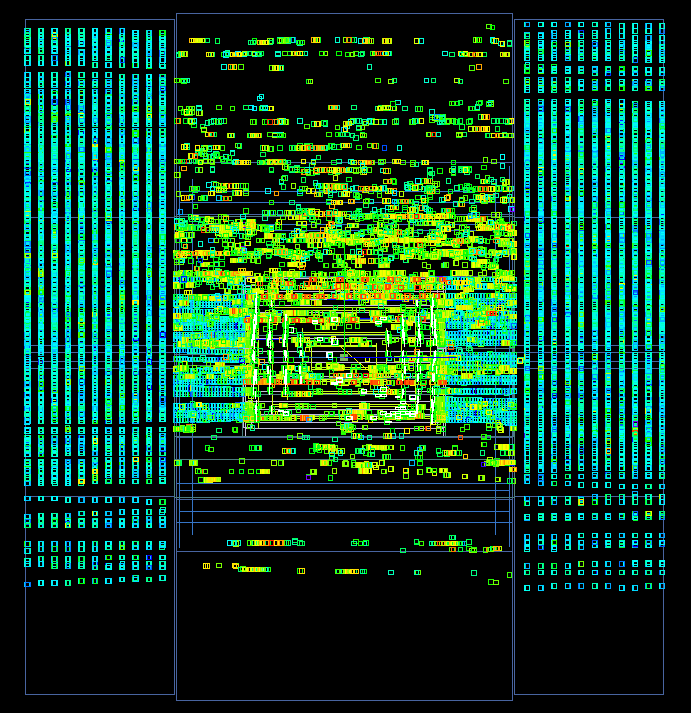
\includegraphics[height=0.3\textheight]{figures/muons_positron_5spoilers_wall_515_zyview_croped.png}
        \caption{xy-view}
        \label{fig:zy_5Spoilers}
    \end{subfigure}
    \caption[Event displays of muons in SiD from the '5 Spoilers' scenario]{
    Event displays in the xy- and zy-view of the muons from the '5 Spoilers' scenario in the SiD detector.
    }
    \label{fig:WIRED4_5Spoilers}
\end{figure}

\begin{figure}
    \centering
    \begin{subfigure}[b]{0.49\textwidth}
    \centering
        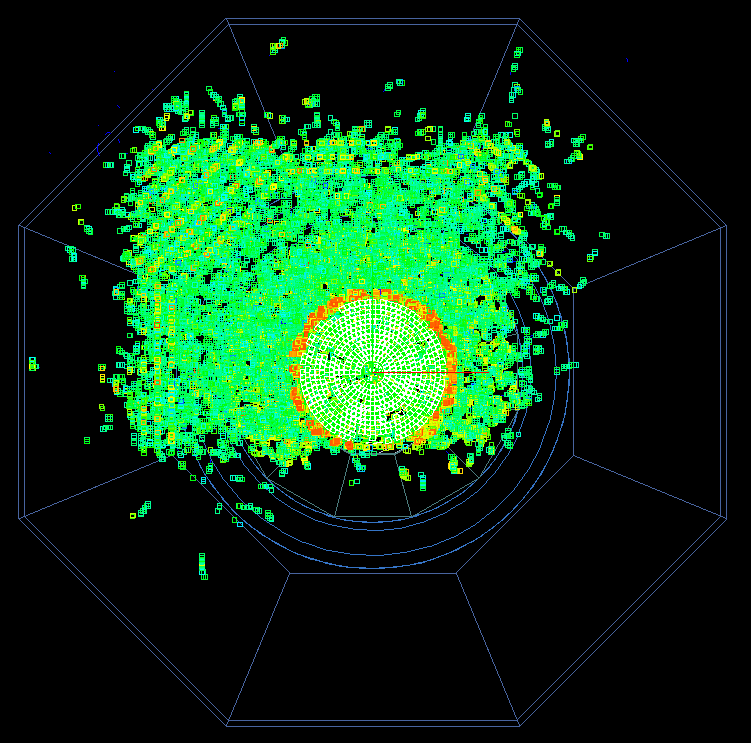
\includegraphics[height=0.3\textheight]{figures/muons_positron_5spoilers_2961_xyview_croped.png}
        \caption{xy-view}
	\label{fig:xy_5SpoilersWall}
    \end{subfigure}
    \begin{subfigure}[b]{0.49\textwidth}
    \centering
        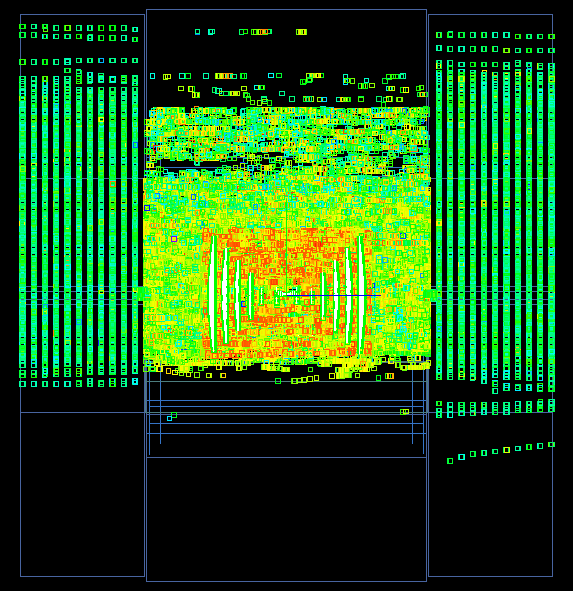
\includegraphics[height=0.3\textheight]{figures/muons_positron_5spoilers_2961_zyview_croped.png}
        \caption{xy-view}
        \label{fig:zy_5SpoilersWall}
    \end{subfigure}
    \caption[Event displays of muons in SiD from the '5 Spoilers + Wall' scenario]{
    Event displays in the xy- and zy-view of the muons from the '5 Spoilers + Wall' scenario in the SiD detector.
    }
    \label{fig:WIRED4_5SpoilersWall}
\end{figure}